% Drawing 71/01-2 -- folder 71, batch 01, archive page 2 (PDF page 3).
% Transcription: à gauche, un croquis tracé la feuille tournée d'un quart de tour : deux régions arrondies accolées, limitées par trois arcs qui joignent deux points — $\Gamma'_1$ à gauche, $\Gamma'_2$ à droite et l'arc médian $\Gamma'_3$ ; le point du haut est entouré d'un petit cercle, celui du bas est noté $y$ ; quatre longs traits obliques hachurent l'ensemble.
% Kind: two regions bounded by three arcs joining two points, small circle round one of them, hatching. Method 2 (schematic redraw from the facsimile). Status: ok.
% Notes: The sketch was drawn with the sheet turned by a quarter turn (its labels read upright when the scan is turned 90 degrees clockwise); the crop is turned that way and the figure redrawn with its labels upright. The three arcs start and end at the same two computed points: the upper one, inside the small circle, and the lower one, labelled y. Labels Gamma'_1 (left, outside), Gamma'_2 (right, outside), Gamma'_3 (beside the median arc). Inside the small circle a small letter (x, as on p. 13) at the upper left and an inked blot at the right; the blot is not drawn. The hatching is four long oblique strokes, drawn as on the page (two end in a hook), and two short dotted arcs. Decided by a machine pass, 2026-11-12: the subscripts of the two outer labels are read 1 (left) and 2 (right) -- the strokes are small, but the text of the page names exactly Gamma'_1, Gamma'_2, Gamma'_3 and the figure of p. 13 has the same layout. Not checked by a reader. The transcription's note (« deux cercles sécants ») describes the same figure; the two outlines are not circles that cross but two lobes sharing the median arc. Redrawn 2026-11-12 (issue 128): to check again.
% Coordinates: 1 unit = 1 mm = 1/100 of the crop width (bbox in page fractions: [0.14, 0.25, 0.32, 0.39]).
% Redrawn by Claude (claude-fable-5-2), issue #128, 2026-11-12; not checked by a human; not compiled (no TeX in the session).
% Rights: reproduces part of the work -- behind RENDER_TRANSCRIPTS, never published by itself.
\documentclass[tikz,border=3pt]{standalone}
\usepackage{amsmath,amssymb}
\usetikzlibrary{patterns,arrows.meta}
\tikzset{pencil/.style={black!45}, struck/.style={black!35}, mpt/.style={circle,draw,inner sep=1.3pt}, pt/.style={circle,fill,inner sep=0.9pt}, opt/.style={circle,draw,fill=white,inner sep=1.1pt}}
\begin{document}
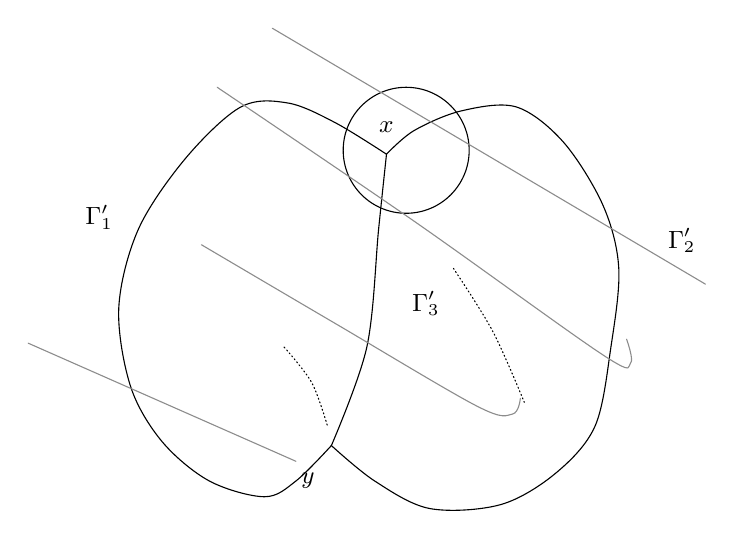
\begin{tikzpicture}[x=1mm,y=1mm,line cap=round,line join=round,font=\scriptsize]
\draw plot[smooth, tension=0.55] coordinates {(46.5,-30.5) (40,-26.5) (34,-24) (28,-24.5) (21,-31) (15,-40) (12.5,-50) (14,-60) (18,-67) (24,-72) (31,-74) (35,-72) (39.5,-67.5)};
\draw plot[smooth, tension=0.55] coordinates {(46.5,-30.5) (50,-27.5) (56,-25) (63,-24.5) (69,-29) (74,-37) (76,-45) (75,-55) (73,-65) (68,-71) (61,-75) (52,-75.5) (45,-72) (39.5,-67.5)};
\draw plot[smooth, tension=0.55] coordinates {(46.5,-30.5) (45.5,-40) (44,-55) (39.5,-67.5)};
\draw (49,-30) circle[radius=8];
\node[inner sep=1pt] at (46.5,-27) {\small $x$};
\node[inner sep=1pt] at (36.5,-72) {\small $y$};
\draw[pencil] (32,-14.5) -- (87,-47);
\draw[pencil] plot[smooth, tension=0.55] coordinates {(25,-22) (50,-39) (74,-56) (77.5,-57) (77,-54)};
\draw[pencil] plot[smooth, tension=0.55] coordinates {(23,-42) (40,-52) (58,-62.5) (62.5,-63.5) (63.5,-61.5)};
\draw[pencil] (1,-54.5) -- (35,-69.5);
\draw[densely dotted] plot[smooth, tension=0.55] coordinates {(33.5,-55) (37,-59.5) (39,-65)};
\draw[densely dotted] plot[smooth, tension=0.55] coordinates {(55,-45) (60,-53) (64,-62)};
\node[inner sep=1pt] at (10,-38.5) {\small $\Gamma'_1$};
\node[inner sep=1pt] at (84,-41.5) {\small $\Gamma'_2$};
\node[inner sep=1pt] at (51.5,-49.5) {\small $\Gamma'_3$};
\end{tikzpicture}
\end{document}
